\subsection{The Commit Dataset}

The \texttt{commit\_survey.csv} dataset provides detailed metadata for over 15,000 Linux kernel commits, including commit types, messages, timestamps, and affected components. It is used to categorize and classify commits, focusing on the eBPF subsystem.

\subsubsection{Dataset Overview}

The dataset contains the following fields:

\begin{itemize}
    \item \textbf{Commit Metadata}: Unique commit IDs, author and committer details, and timestamps.
    \item \textbf{Commit Messages and File Changes}: Descriptions of the changes in each commit.
    \item \textbf{Classification}: Types such as bug fixes, feature additions, or merges.
    \item \textbf{Complexity}: Based on the number of files and lines changed.
    \item \textbf{Components}: Affected implementation and logic components.
    \item \textbf{Use Cases}: Related subsystems and modules.
\end{itemize}

% References
% \bibliographystyle{IEEEtran}
% \bibliography{references}

\paragraph{Commit Classification Distribution}

\begin{figure}[ht]
    \centering
    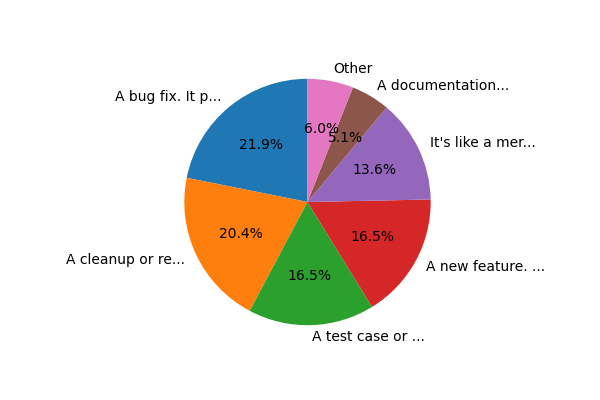
\includegraphics[width=\linewidth]{feature-analysis/commit_pie_chart_commit_classification.png}
    \caption{Commit Classification Distribution}
    \label{fig:commit_pie_chart_commit_classification}
\end{figure}

Most commits focus on bug fixes and code cleanups, reflecting ongoing efforts to maintain code quality. Significant attention is also given to testing infrastructure changes, emphasizing the importance of robustness. New features constitute a considerable portion of the commits, while merge commits are commonplace in the Linux kernel's development process.

\paragraph{Commit Complexity Distribution}

\begin{figure}[ht]
    \centering
    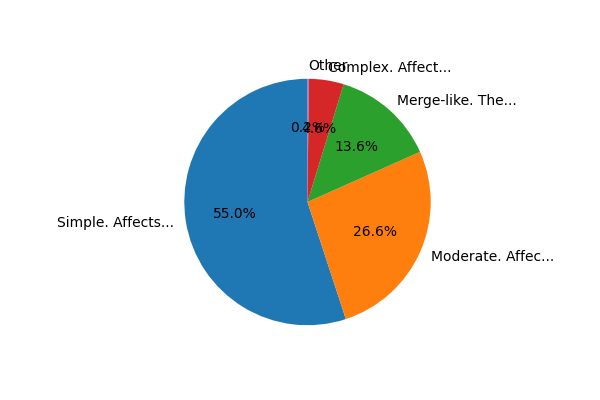
\includegraphics[width=\linewidth]{feature-analysis/commit_pie_chart_commit_complexity.png}
    \caption{Commit Complexity Distribution}
    \label{fig:commit_pie_chart_commit_complexity}
\end{figure}

The majority of commits are simple, involving small changes, while more complex changes constitute a smaller but noteworthy portion.

\paragraph{Major Related Implementation Components}

\begin{figure}[ht]
    \centering
    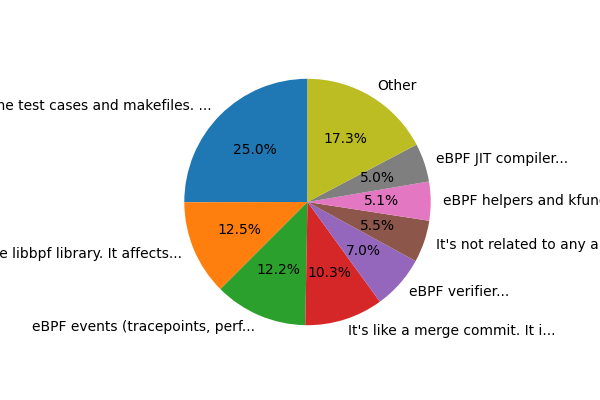
\includegraphics[width=\linewidth]{feature-analysis/commit_pie_chart_major_implementation_component.png}
    \caption{Major Related Implementation Components}
    \label{fig:commit_pie_chart_major_implementation_component}
\end{figure}

Test cases and build scripts are significantly affected, highlighting continuous improvements in testing and build processes. The \texttt{libbpf} library is also a key component in the kernel eBPF toolchain, receiving considerable development attention. Additionally, substantial development occurs in other kernel subsystems, particularly related to eBPF events. The frequent updates to the eBPF verifier and helpers indicate ongoing efforts to enhance functionality and ensure program safety. Notably, some commits appear unrelated to the eBPF subsystem.

\paragraph{Logic Components Affected}

\begin{figure}[ht]
    \centering
    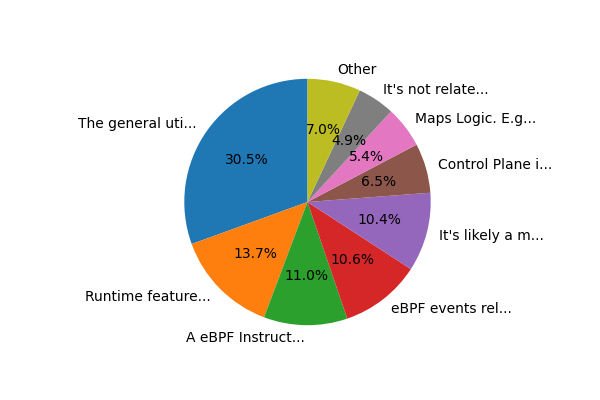
\includegraphics[width=\linewidth]{feature-analysis/commit_pie_chart_major_logic_component.png}
    \caption{Major Related Logic Components}
    \label{fig:commit_pie_chart_major_logic_component}
\end{figure}

General utilities, such as tools and scripts, receive the most updates, followed by runtime features like helpers and kernel functions, which are consistently enhanced. eBPF event logic and instruction handling are also frequently updated to ensure robustness and functionality.

\paragraph{Use Cases and eBPF Events}

\begin{figure}[ht]
    \centering
    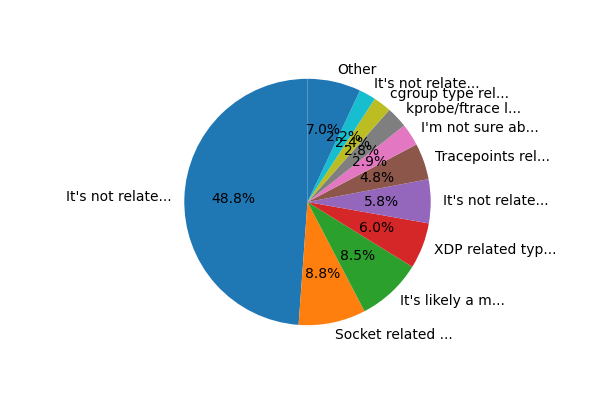
\includegraphics[width=\linewidth]{feature-analysis/commit_pie_chart_usecases_or_submodule_events.png}
    \caption{Related Events and Use Cases}
    \label{fig:commit_pie_chart_usecases_or_submodule_events}
\end{figure}

While most commits enhance the core eBPF infrastructure—including the verifier and runtime components—significant development also extends to networking-related features such as socket and XDP programs, which receive substantial attention. Additionally, tracing tools like tracepoints and kprobes highlight eBPF's crucial role in system diagnostics and debugging.